%
%   latex writeup for KeystrokeAuth
%   6.858 Final Project
%   December 2013
%   forrestp, ameeshg, kseibert, cbieden
%
%

\documentclass{article}

\usepackage{geometry}
\geometry{letterpaper}

\usepackage{doc}

\usepackage{graphicx}
\usepackage{float}
\usepackage{caption}
\usepackage{subcaption}

\usepackage{epstopdf}

\usepackage{enumitem}
\setdescription{leftmargin=\parindent,labelindent=1cm}

\title{KeystrokeAuth}
\author{
  Forrest Pieper\\
  Kenneth Seibert\\
  Ameesh Goyal\\
  Carlo Biedenharn
}
\date{December 10th, 2013}

\begin{document}

\maketitle

\abstract{
}

\section{Introduction}
\label{introduction}
KeystrokeAuth is an example website implementation that uses keystroke timing to provide stronger user authentication.
Measuring keystroke timing is a method for passive biometric authentication. 
Traditional biometric authentication such as fingerprint or retinal scanners require external hardware and is not suited for web service authentication where users may login from a variety of machines. 
Keystroke timing can be gathered using javascript embedded in the login and registration pages.
Thus this method requires no additional hardware.
The user must enter her password several times during registration instead of just once or twice, but other than that this method is completely unobtrusive.
Authenticating passwords with keystroke timing makes it more difficult for an attacker who possesses a user's plaintext password to compromise the account.
Additionally, it discourages account sharing which may be useful for highly secure systems and premium accounts.
In this paper we describe past work on the topic, introduce our example implementation called KeystrokeAuth, analyze the added security of our system, and examine a small set of test data.

\section{Background and Related Work}
TODO: forrest / carlo / kenny / ameesh
Many different studies have been done in the past about fingerprinting users based on keystroke cadence, a few of which are referenced below. However, many of these studies focus on running a keylogger in the background of a user session and collecting a large amount of keystrokes before making a decision. The model that these keystrokes are compared to can also be quite large. In contrast, KeystrokeAuth can only compare the timing data from a short password entry to the timing data of a small bank of previously entered passwords. This makes detecting adversaries much more difficult.

In our system, we avoided the legwork of comparing multiple algorithms for what may be the best fit for us. Instead, we chose a few of the top performing algorithms described in \[1\] to test in a password context. 

describe various detectors

\section{KeystrokeAuth Implementation}
KeystrokeAuth uses javascript to capture the timestamps on each keydown and keyup event while typing the password.
During registration, the user enters her password 10 times.
The data is sent to the server and KeystrokeAuth computes a model specific to that user and password.
When logging in, the user enters the password once and KeystrokeAuth compares the new timing data to the registered model.
If the timing data differs by too much, the user will not be logged in.

\subsection{Gathering Timing Data}
TODO: forrest

Gather code, uptime, downtime --> compute various features

\subsection{Generating User Timing Model}
In order to have success with verifying users using keystroke dynamics, we first have to collect a set of training data. The keystroke dynamics that we are interested in include down time, down-down time, flight time, and dwell time which are defined below. 
\begin{description}
	\item[Down time:] The time that each key is pressed down at, where the first key pressed down equates to a time of zero
	\item[Down-Down time:] The time in-between two consecutive key down events
	\item[Flight time:] The time in-between a key up and the following key down event. This value can be negative as a key may not be released before the next is pressed down. 
	\item[Dwell time:] The time that a given key is held down
\end{description}
We are able to calculate all of these values from the initial 10 password entries that are passed in during registration. The calculated data is then encrypted with AES CFB encryption using a salted and hashed (PBKDF2) user password as the key. The salt in this case differs from the salt and hash of the user password that is stored on the server. Thus, for each user, the server stores the username, two different salts, the hashed and salted password, and the encrypted timing data.

These metrics will be used when a login attempt is received to determine whether or not to authenticate a given user.

\subsection{Login Timing Authentication}
In order to determine whether or not the user attempting to log in should be authenticated, we collect the down time, the down-down time, the flight time, and the dwell time to compare against the training data. We make use of the mahalanobis distance to compute the similarity between two vectors.  \\
\begin{displaymath}
D_m(\vec{x}) = \sqrt{(\vec{x}-\vec{y})^T S^{-1} (\vec{x}-\vec{y})}
\end{displaymath} \\
We make use of the mahalanobis distance in both of authentication functions. The first function we use takes the mean of the training data vectors and computes the distance between the login attempt and the computed mean vector. If the distance from the mean vector is below a certain threshold, then the login attempt is accepted. The 2nd function that we employ is we take the login attempt and find its distance from each of the training vectors. If the $k$ closes distances all fall below a threshold, then the login attempt is accepted. \\ \\
The threshold is computed using the training data. We find the mahalanobis distance between each vector in the training data. We then compute the average distance. The threshold is set to be one deviation away from the mean in the direction of smaller distances. In other words we only accept login attempts where the distance of the attempt is at least one deviation than our computed mean distance. 
\section{Security Analysis}
TODO: forrest

proof that security is not worse

strategy: make it no less convenient/difficult for users, and at least slightly more secure

\section{Data Collection and Analysis}

\subsection{Data Overview}
Timing data was recorded from twelve participants typing three phrases. In an effort to record relevant data while not divulging the passwords of the participants, familiar phrases were used. Each participant was instructed to type each phrase at least ten times, in any order. Each participant had to type the same three phrases: \textit{facebookgoogle}, \textit{phideltatheta}, and \textit{biedenharn}.\\

The phrase \textit{facebookgoogle} was chosen as it is universally familiar to our participants, resulting in very consistent typing rhythms. \textit{phideltatheta} was used because a portion of our participants were familiar with the phrase. The last phrase, \textit{biedenharn}, was chosen as an example of an attack where \textit{biedenharn} was the account password of a user and the participants were trying to compromise the account. Like a password, \textit{biedenharn} was not familiar to any of our participants except for one of the authors of this paper.\\

Even when looking at the messy graph in Figure \ref{full_facebookgoogle_flight}, it is clear that individuals have unique typing rhythms with familar words. Filtering the data down to a few participants in Figure \ref{multi_facebookgoogle_flight} shows this more directly.

\begin{figure}[H]
  \begin{subfigure}[b]{75mm}
    \centering
    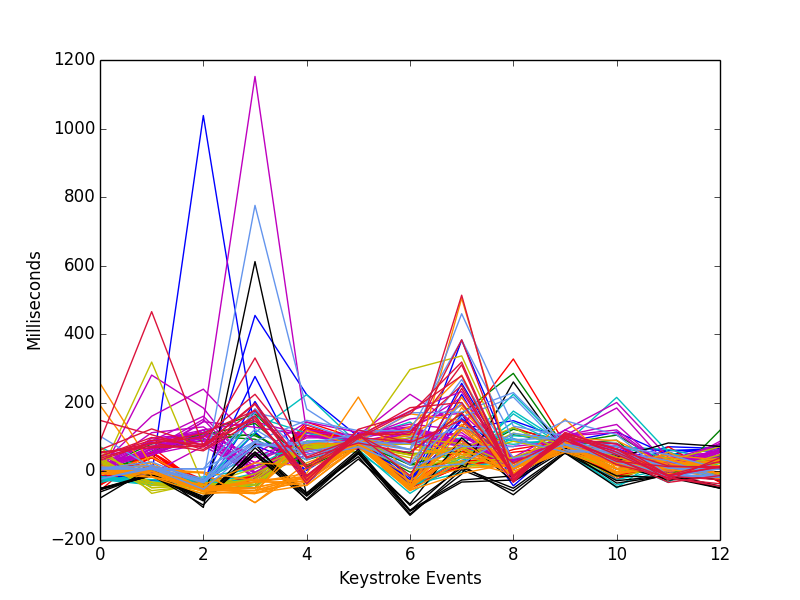
\includegraphics[width=70mm]{facebookgoogle_flight_final.png}
    \caption{All data}
    \label{full_facebookgoogle_flight}
  \end{subfigure}
  \begin{subfigure}[b]{75mm}
    \centering
    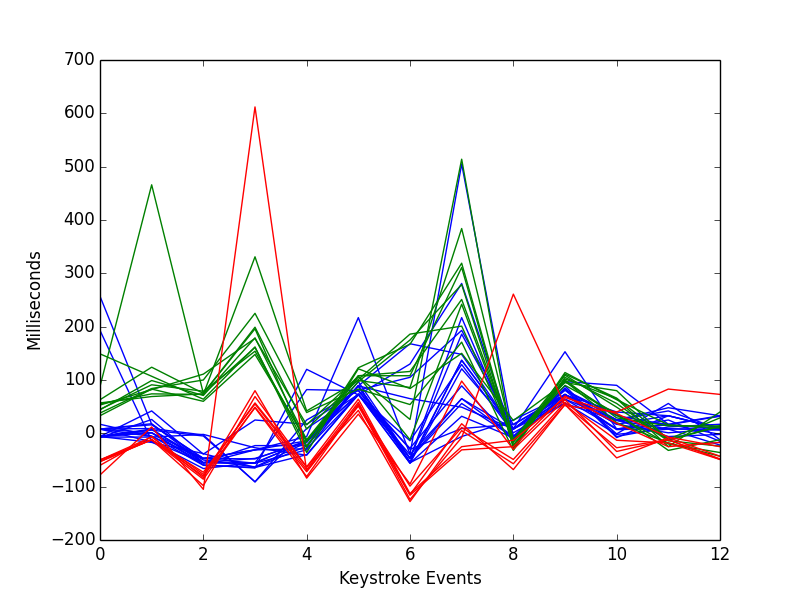
\includegraphics[width=70mm]{facebookgoogle_multi_flight_final.png}
    \caption{Three individuals}
    \label{multi_facebookgoogle_flight}
  \end{subfigure}
  \caption{Flight measurements for participants typing \textit{facebookgoogle}. Each distinct color represents an individual.}
\end{figure}

\subsection{Feature Comparison} 

In practice, the different features produce variably unique datasets. Though the graphs comparing the \textit{up} and \textit{down} features are unique, it is easy to see in figure \ref{all_graphs:down} that with practice an attacker might be able to replicate a victim's data. However with the \textit{flight} and \textit{down-down} graphs (figures \ref{all_graphs:flight} and \ref{all_graphs:down-down}), the results are very consistent and unique. The green dataset has mostly positive flight times while the blue dataset has mainly negative times.

\begin{figure}[H]
  \centering
  \begin{subfigure}[b]{0.3\textwidth}
    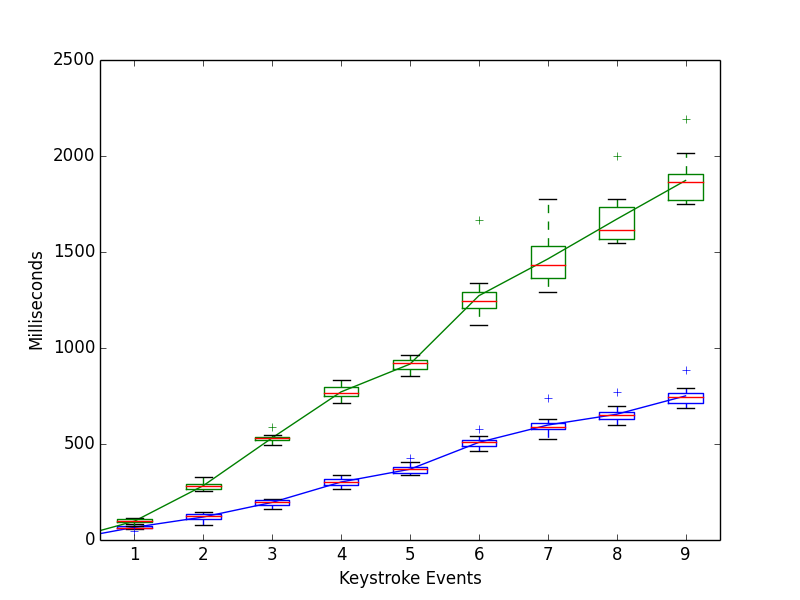
\includegraphics[width=\textwidth]{biedenharn_jordan_down_final.png}
    \caption{down}
    \label{all_graphs:down}
  \end{subfigure}%
  ~ %add desired spacing between images, e. g. ~, \quad, \qquad etc.
    %(or a blank line to force the subfigure onto a new line)
  \begin{subfigure}[b]{0.3\textwidth}
    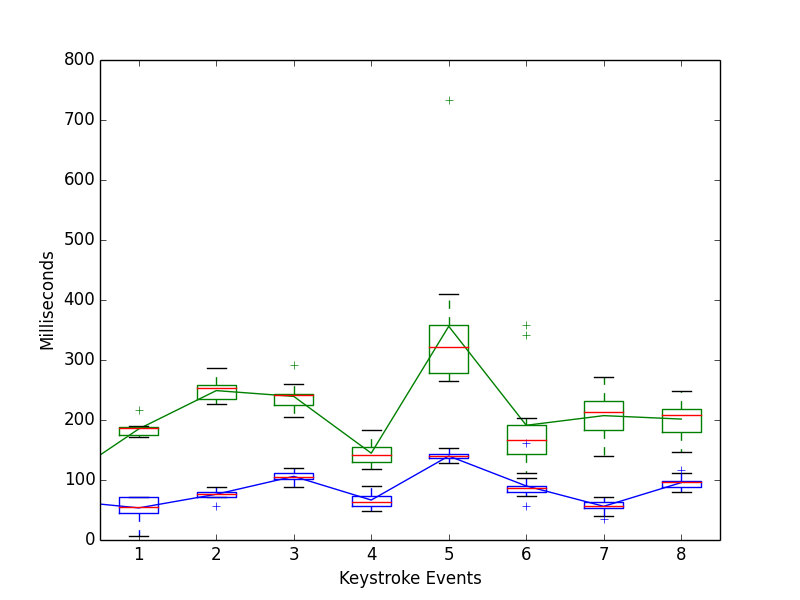
\includegraphics[width=\textwidth]{biedenharn_jordan_down-down_final.png}
    \caption{down-down}
    \label{all_graphs:down-down}
  \end{subfigure}
  ~ %add desired spacing between images, e. g. ~, \quad, \qquad etc.
    %(or a blank line to force the subfigure onto a new line)
  \begin{subfigure}[b]{0.3\textwidth}
    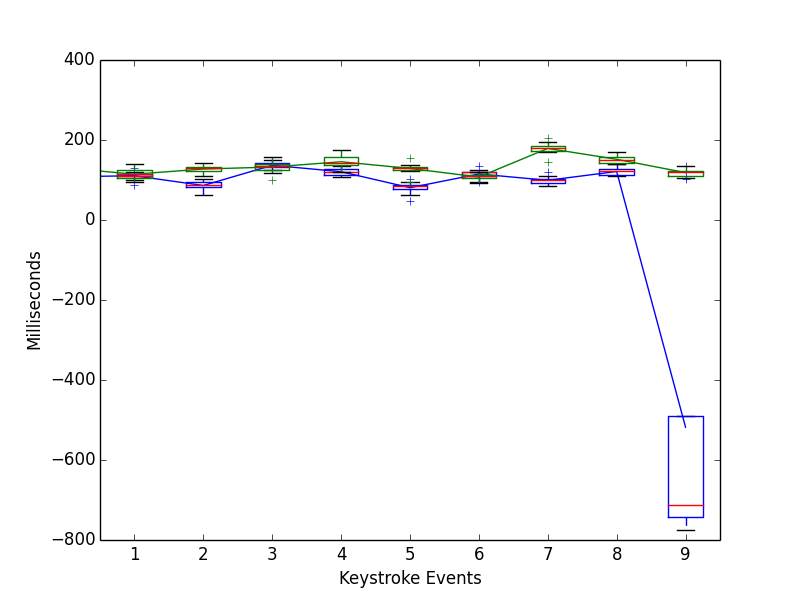
\includegraphics[width=\textwidth]{biedenharn_jordan_dwell_final.png}
    \caption{dwell}
    \label{all_graphs:dwell}
  \end{subfigure}

  \begin{subfigure}[b]{0.3\textwidth}
    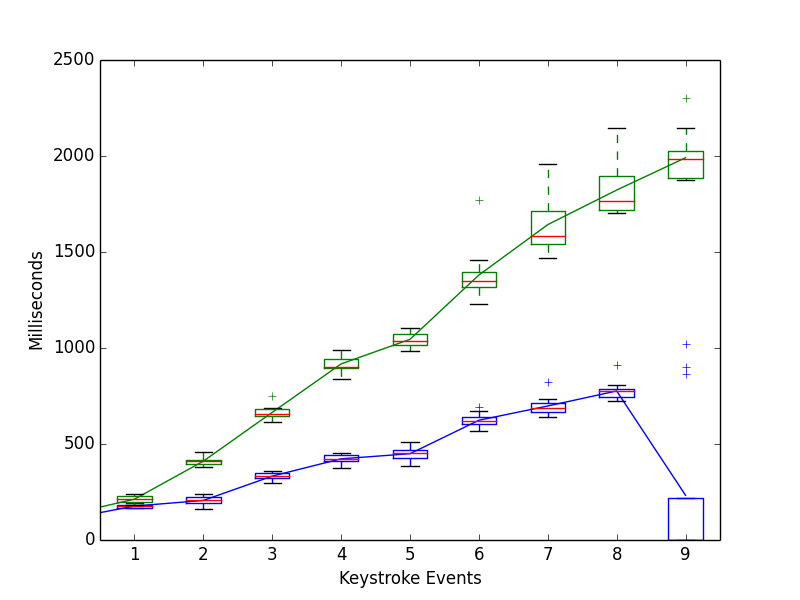
\includegraphics[width=\textwidth]{biedenharn_jordan_up_final.png}
    \caption{up}
    \label{all_graphs:up}
  \end{subfigure}%
  ~ %add desired spacing between images, e. g. ~, \quad, \qquad etc.
    %(or a blank line to force the subfigure onto a new line)
  \begin{subfigure}[b]{0.3\textwidth}
    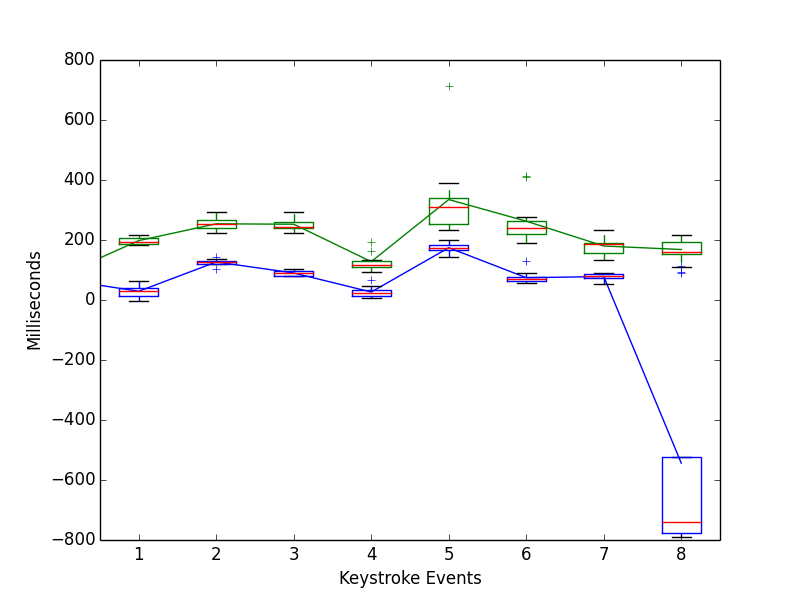
\includegraphics[width=\textwidth]{biedenharn_jordan_up-up_final.png}
    \caption{up-up}
    \label{all_graphs:up-up}
  \end{subfigure}
  ~ %add desired spacing between images, e. g. ~, \quad, \qquad etc.
    %(or a blank line to force the subfigure onto a new line)
  \begin{subfigure}[b]{0.3\textwidth}
    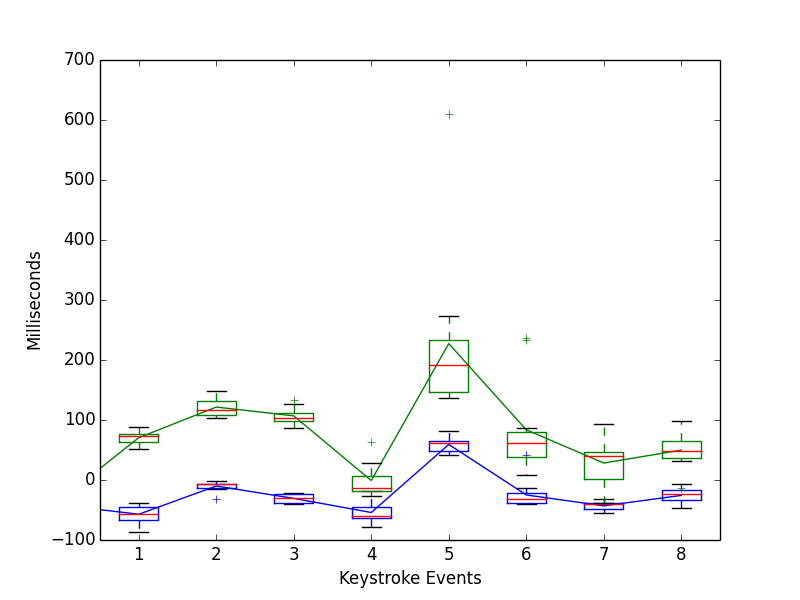
\includegraphics[width=\textwidth]{biedenharn_jordan_flight_final.png}
    \caption{flight}
    \label{all_graphs:flight}
  \end{subfigure}
  \caption{Comparison of the six features. The blue data represents the phrase \textit{biedenharn} typed by somebody familiar with the phrase. The green data represents somebody unfamilar with the phrase.}
  \label{all_graphs}
\end{figure}

\subsection{Error Rates}    %false positive (someone else logs in) and false negative (I can't log in)

Goal: Find ideal thresholds and weights for each feature that give 1\% false negative rate
ideal would be  .001\% false positive, but anything less than 100\% is an improvement over state of the art
Compromise: increase false positive rate to accommodate 1\% false negative

\section{Conclusion}
TODO: forrest / carlo / kenny / ameesh


\begin{thebibliography}{99}
  \bibitem{Killourhy09}
    %comparison of various keystroke timing schemes
   Killourhy, Kevin S., and Roy A. Maxion. 
   ``Comparing anomaly-detection algorithms for keystroke dynamics.''
   \textit{Dependable Systems \& Networks, 2009. DSN'09. IEEE/IFIP International Conference on.}
   IEEE, 2009. 
 
 \bibitem{Cho00}
    %Nearest-neighbor mahalanobis
   Cho, Sungzoon, et al.
   ``Web-based keystroke dynamics identity verification using neural network.'' 
   \textit{Journal of organizational computing and electronic commerce}
   10.4 (2000): 295-307.
  
\end{thebibliography}

\end {document}
